\documentclass[12pt]{article}
\usepackage[a4paper,left=1in,right=1in]{geometry}
% marginleri 1er inch yaptim, isterseniz daha da arttirabiliriz.
\renewcommand{\baselinestretch}{1.15} % satir araligi 1.15
\usepackage{mathptmx}
\usepackage[utf8]{inputenc}
\usepackage[style=ieee]{biblatex}
\usepackage[document]{ragged2e}
% \usepackage{amsmath}
\usepackage{graphicx}
\graphicspath{{./images/}}
% \usepackage{makeidx}
% \usepackage{rotating}
% \usepackage{tikz}
\usepackage{acronym}
\usepackage{hyperref}
% \usepackage{float}
\usepackage{caption}
\usepackage{filecontents}
\captionsetup[table]{name=Tablo}
\renewcommand{\figurename}{Şekil}
\renewcommand{\contentsname}{İçindekiler}
\addbibresource{references.bib}
%\renewcommand\refname{New Title}
% \selectlanguage{turkish}
\newcommand{\HRule}[1]{\rule{\linewidth}{#1}}
%\newcommand{\HRule}{\rule{\linewidth}{0.5mm}} 
\begin{document}




\title{\vspace{1cm}


\textsc{\LARGE TEKNOFEST}\\[0.5cm]
\textsc{\large HAVACILIK, UZAY VE TEKNOLOJİ FESTİVALİ}\\[0.5cm]
\textsc{\large İnsansız Su Altı Sistemleri Yarışması}\\[0.5cm]
\HRule{0.5pt} \\[0.4cm]
{\LARGE \bfseries ÖN TASARIM RAPORU}\\[0.3cm]
\HRule{0.5pt} \\[1.0cm]
%{\large \bfseries Ön Tasarım Raporu}\\[1cm]

%\includegraphics{logo.png}\\[1cm]
\date{}
\author{
\textbf{Takım Adı}       &   Nucleo\\[10pt]
\textbf{Takım ID}        &   T3-16167-166\\[10pt]
\textbf{Takım Üyeleri}   &   Ege Saygılı, Enes Demirağ, Sencer Yazıcı, Sinan Ertuğrul Yıldırım\\[10pt]
\textbf{Takım Danışmanı} &   Ar. Gör. Mehmet Ozan Şerifoğlu 
}
}
\maketitle
\newpage
\tableofcontents

\newpage
\addcontentsline{toc}{section}{Kısaltmalar}
\section*{Kısaltmalar}
\begin{acronym}[Nucleo] 
%\acro{KISTALTMA}{ACIKLAMA / %\textit{INGILIZCESI}}
% ALFABETİK YAPILDI
\acro{3B}{Üç Boyutlu}
\acro{AUV}{Otonom Su Altı Aracı / \textit{Autonomous Underwater Vehicle}}
\acro{AWG}{Amerikan Kablo Ölçüsü / \textit{American Wire Gauge}}
\acro{CFD}{Hesaplamalı Akışkanlar Dinamiği / \textit{Computational Fluid Dynamics}}
\acro{ESC}{Elektronik Hız Kontrolcüsü / \textit{Electronic Speed Controller}}
\acro{GUI}{Grafiksel Kullanıcı Arayüzü / \textit{Graphical User Interface}}
\acro{HD}{Yüksek Çözünürlük / \textit{High Definition}}
\acro{IP}{İnternet Protokolü / \textit{Internet Protocol}}
\acro{openCV}{\textit{Open Source Computer Vision Library}}
\acro{PCB}{Baskı Devre Kartı / \textit{Printed Circuit Board}}
\acro{PID}{Oran-İntegral-Türev / \textit{Proportional-Integral-Derivative}}
\acro{PMMA}{Akrilik / \textit{Poly (Methyl Methacrylate)}}
\acro{PWM}{Sinyal Genişlik Modülasyonu / \textit{Pulse Width Modulation}}
\acro{Rqt}{ROS Qt Görsel Araçları / \textit{Ros Qt Widgets}}
\acro{ROS}{Robot İşletim Sistemi / \textit{Robot Operating System}}
\acro{ROV}{Uzaktan Kontrollü Su Altı Aracı / \textit{Remotely Operated Underwater Vehicle}}
\acro{SID}{Sistem Entegrasyon Diyagramı / \textit{System Integration Diagram}}
\acro{UART}{Evrensel Asenkron Alıcı-Verici / \textit{Universal Asynchronous Receiver-Transmitter}}
\acro{USB}{Evrensel Seri Veriyolu / \textit{Universal Serial Bus}}
\acro{WBS}{İş Dağılım Yapısı / \textit{Work Breakdown Structure}}
\end{acronym}


\newpage

\section{Rapor Özeti}

% nucleo ROV mu diyelim? 
\paragraph{} Nucleo, İstanbul Teknik Üniversitesi, Elektrik-Elektronik Fakültesi bünyesindeki farklı bölümlerden dört, son sınıf öğrencisinin bir araya gelerek uzaktan kumandalı sualtı aracı (ROV) gerçekleştirmek üzere kurduğu bir proje takımıdır.

\paragraph{} Takım üyeleri 2017 yılından bu yana İTÜ ROV Takımı ve İTÜ AUV Takımı bünyesinde yorulmak bilmeyen çalışmaların ve edinilen tecrübelerin ardından  yeni bir araç üreterek Teknofest Su altı Sistemleri Yarışması'nda derece elde etmeyi amaçlamaktadır.

\paragraph{} Geliştirilecek araç, su altında yüzeydeki kontrol istasyonundan bir pilotun kontrolü ile veya tamamen otonom olarak çeşitli görevleri yapabilecektir. Araç, Teknofest Su altı Sistemleri Yarışması’nın beklentilerini amaçlanan maksimum başarı düzeyinde gerçekleştirmek üzere tasarlanacak ve üretilecektir. Takımımız, belirli görevlere odaklanmak üzere mekanik, elektronik, ve yazılım olmak üzere üç alt ekibe bölünmüştür. ROV, görev gereksinimlerini yerine getirirken hem minimum boyut hem de ağırlık optimizasyonu ile tasarlanacaktır.

\paragraph{} ROV mümkün olduğunca üniversite bünyesinde üretilebilecek şekilde tasarlanacaktır ve üretim maliyetini en aza indirmek için ekibimizdeki insanların aynı zamanda çalışmakta olduğu İTÜ Gemi İnşaatı ve Deniz Bilimleri Fakültesi'ndeki Otonom Su Altı Aracı (AUV) Takımı'nın çalışma odası kullanılacaktır.

\paragraph{} İTÜ ROV Takımı ve İTÜ AUV Takımı'nın kurucu üyeleri olarak her zaman açık kaynaklı çalışarak su altı sistemleri topluluğuna fayda sağladık. Geçtiğimiz yıllarda geliştirdiğimiz araçlarımız ile ilgili tüm mekanik-elektronik tasarımlar ve yazılımımızı GitHub adresimizde bulabilirsiniz.

\newpage

\section{Takım Şeması}
\subsection{Takım Üyeleri}

\paragraph{} Tüm üyelerimiz İstanbul Teknik Üniversitesi 4. Sınıf öğrencisidir. Takım Danışmanımız Ar. Gör. Mehmet Ozan Şerifoğlu'dur.

\begin{table}[h]
\centering
\resizebox{\textwidth}{!}{%
\begin{tabular}{|l|l|l|}
\hline
\textbf{İsim Soyisim}  & \textbf{Bölüm}                        & \textbf{Çalışma Alanı} \\ \hline
Ege Saygılı             & Kontrol ve Otomasyon Mühendisliği     & Mekanik                \\ \hline
Enes Demirağ            & Elektronik ve Haberleşme Mühendisliği & Organizasyon           \\ \hline
Sencer Yazıcı           & Kontrol ve Otomasyon Mühendisliği     & Yazılım                \\ \hline
Sinan Ertuğrul Yıldırım & Elektrik Mühendisliği                 & Elektronik             \\ \hline
\end{tabular}%
}
\caption{Takım Üyeleri}
\label{tab:takim-uyeleri}
\end{table}

\subsection{Organizasyon Şeması ve Görev Dağılımı}

\paragraph{} Nucleo Takımı, İstanbul Teknik Üniversitesi Elektronik ve Haberleşme Mühendisliği, Kontrol ve Otomasyon Mühendisliği, Elektrik Mühendisliği bölümleri öğrencileri tarafından oluşturulmuştur. Ekip ve proje yönetimini sağlamak için haftalık takım toplantıları yaparken, proje yönetimine yardımcı olmak için planlarımızı Slack uygulaması ile gerçekleştirdik.

\paragraph{} Takımımız az sayıda insandan oluşması nedeniyle, görev dağılımı yapılmış olsa da tüm üyelerin aracın her aşamasında ortak emeği olacaktır. Her üyenin bireysel olarak sorumlu olduğu görevler bulunmaktadır. Ekip üyelerimizden Enes Demirağ takımın genel organizasyonu ve görüntü işleme ve haberleşme sistemleri ile, Sencer Yazıcı otonom navigasyon ve kontrolör tasarımı ile, Ege Saygılı mekanik tasarım ve üretim, Sinan Ertuğrul Yıldırım elektronik devre tasarımı ve güç sistemleri üzerinde çalışmaktadır.

\newpage

\section{Araç Ön Tasarımı}


\paragraph{} Takımımızın ROV sistemi yüzeyde bulunan bir kontrol istasyonu, ve ROV'un kendisinden oluşmaktadır. Kontrol istasyonunda 15.6 inçe kadar dizüstü bilgisayar kullanımı desteklenmektedir. Aynı zamanda yüzey kontrol istasyonunda 12VDC 20A kapasiteli ROV'nin güç kaynağı bulunmaktadır, güç kaynağı ile ROV güç beslemesi arasında 20A bir sigorta bulunmaktadır. Taşınabilir yüzey istasyonunu prize bağlanması ve ROV'unda yüzey istasyonuna bağlanmasının ardından ROV kullanıma hazır olmaktadır.

\paragraph{} ROV üzerinde beş eksende hareket özgürlüğü sağlaması için altı adet fırçasız motorlu itici bulunmaktadır. İticiler takımımız tarafından tasarlanmıştır. ROV'un elektronikleri su geçirmez akrilik bir kap içerisinde bulunmaktadır. Su geçirmez kaba kablo girişleri/çıkışları, kapak sistemleri vs. tüm su girişi olabilecek açıklıklarda o-ring conta sistemi kullanılmıştır. 

\newpage
\subsection{Sistem Ön Tasarımı}

\begin{figure}[h]
\centering
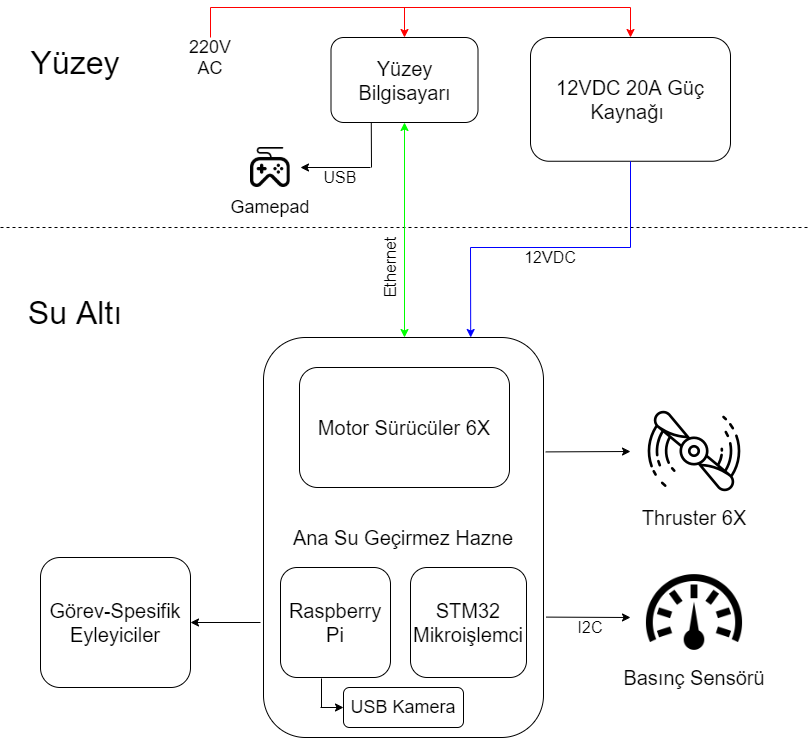
\includegraphics[width=1\textwidth]{SID.png}
\caption{System Integration Diagram}
\end{figure}

\paragraph{} AUV, su altında herhangi bir kontrol veya komuta sistemine bağlı kalmadan, yüksek çözünürlüklü algılayıcılar ve kameralar yardımı ile hareket sistemini kullanarak önceden belirlenmiş görevleri, daha önce tanımadığı bir ortamda otonom bir şekilde gerçekleştirebilen bir su altı aracıdır. Tasarım sürecinde olan aracımızın tasarım gerekçeleri teknik özellikler kısmında açıklanacaktır.
\newpage
\subsection{Aracın Mekanik Tasarımı}

\subsubsection{Mekanik Tasarım Süreci}

\paragraph{} AUV, su altında herhangi bir kontrol veya komuta sistemine bağlı kalmadan, yüksek çözünürlüklü algılayıcılar ve kameralar yardımı ile hareket sistemini kullanarak önceden belirlenmiş görevleri, daha önce tanımadığı bir ortamda otonom bir şekilde gerçekleştirebilen bir su altı aracıdır. Tasarım sürecinde olan aracımızın tasarım gerekçeleri teknik özellikler kısmında açıklanacaktır.

\subsubsection{Malzemeler}

\paragraph{} Aracın iskeletini oluşturan parçalar ve su geçirmez haznenin tüpü gibi parçalar akrilik (PMMA) malzemeden seçilmiştir. Akrilik, hazır tüp bulunmasının kolaylığı, plaka halinde bulunmasının kolaylığı, lazer kesiminin çok kolay bulunuyor olması, ekonomik olması ve görsel özellikleri gibi sebeplerden dolayı seçilmiştir. İtici motorların koruyucu kısımları, pervaneler ve tutucu manipülatör gibi parçalar 3B plastik basım yöntemiyle üretilecektir. Su geçirmez haznenin o-ring conta bulunduran flanş parçaları alüminyumdan seçilmiştir. Araçta sabitleme elemanı olarak paslanmaz alyan başlı civatalar, paslanmaz somun ve gijonlar kullanılacaktır.

\subsubsection{Üretim Yöntemleri}


\paragraph{} Aracın şasesini oluşturan akrilik parçalar lazer kesim yöntemi ile işlenecektir. Bu yöntem ve akrilik malzeme seçimi üretim kolaylığı ve ekonomik oluşundan dolayı tercih edilmiştir. Su geçirmez kabın contalı flanşı aluminyumdan manuel torna da talaşlı imalat yöntemiyle işlenecektir. 3B plastik parçalar 3B yazıcılar yardımıyla basılacaktır.\newpage

\subsubsection{Fiziksel Özellikler}

\begin{figure}[h]
\centering
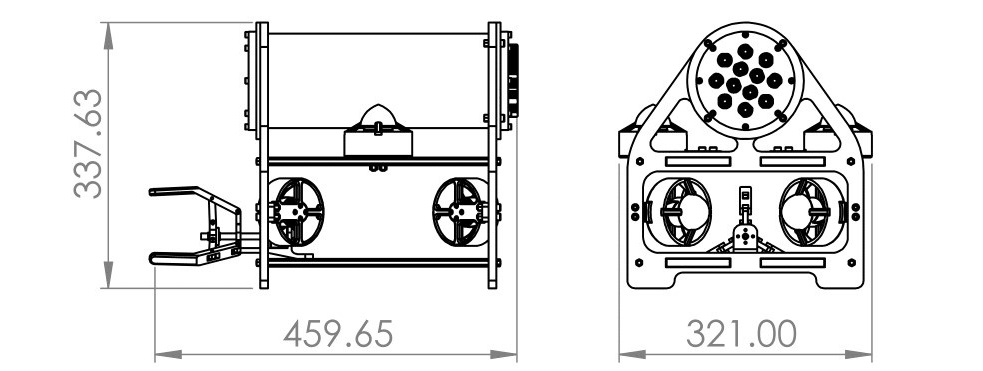
\includegraphics[width=1\linewidth]{specs.jpg}
\caption{Su Altı Aracının Ölçüleri}
\end{figure}


\paragraph{} Aracın ölçüleri 32cm genişlik, 34cm yükseklik ve 46cm uzunluk şeklindedir. Aracın ağırlığı ve yüzerliği 6.8kg dır, bu sayede araç hafifçe pozitif bir yüzerliğe sahiptir, herhangi bir kontrol kaybında araç hafif yüzerliği sayesinde yüzeye çıkacak ve sudan geri alınabilecektir. 


\subsection{Elektronik, Algoritma ve Yazılım Tasarımı}

\subsubsection{Elektronik Ön Tasarım Süreci}

\paragraph{} Blabla


\subsubsection{Algoritma Ön Tasarım Süreci}


\paragraph{} Blabla


\subsubsection{Yazılım Ön Tasarım Süreci}


\paragraph{} Blabla


\subsubsection{Dış Arayüzler}


\paragraph{} Blabla


\section{Güvenlik}


\paragraph{} Aracımızın tasarımı gibi teknik, üretim ve montaj gibi pratik işlerin yanısıra en büyük önceliğimiz iş güvenliği ve emniyetdir. Testlerde, atölye çalışmalarında, önceliğimiz çalışmak için güvenli ve konforlu alanı oluşturmak olacaktır. Takım olarak, ekip üyelerine herhangi bir zarar gelmemesi ve olası iş kazalarını önlemek için her türlü önlemi uygulamaktan çekinmeyeceğiz.
Atölye çalışmalarımızda kişisel koruyucu ekipmanlar olan gözlük, eldiven, maske gibi ekipmanların kullanılmasının yanında atölyemizde acil göz banyosu ve ilk yardım kiti bulundurmayı da ihmal etmedik. Tüm çalışma alanlarımızda uyarı levhaları kullandık.

\paragraph{} Aracımızın teknik özelliklerine dikkat ederken, güvenlik önlemlerini de göz ardı etmedik. Aracın üzerindeki motorların yerleşimi dışarıdan zarar gelmeyecek ve dışarıya zarar vermeyecek şekilde konumlandırıldı. Bunların yanında, aracın üzerindeki tüm plastik kelepçeler kullanıcılara zarar veremeyecek şekilde tıraşlanmıştır. Aracın üzerinde hiçbir sivri yüzey bırakılmamıştır. Aracın su altında herhangi bir sorunda karşılaşılması durumunda karadaki kontrol merkezinde bulunan acil durdurma butonu sayesinde aracı hızlı bir şekilde durdurabilme imkanımız bulunmaktadır. Ayrıca araç üzerindeki manipülatörlerin, operasyon esnasında pilotun kontrol merkezinden gücünün kesilmesi mümkündür.


\section{Zaman, Bütçe ve Risk Planlaması}

\paragraph{} Blablabla

\begin{table}[h]
\centering
\resizebox{\textwidth}{!}{%
\begin{tabular}{|l|c|r|r|}
\hline
\multicolumn{1}{|c|}{\textbf{Malzeme İsmi}} & \textbf{Adet} & \multicolumn{1}{c|}{\textbf{Fiyat}} & \multicolumn{1}{c|}{\textbf{Toplam Fiyat}} \\ \hline
iBM2208Q BLDC Motor      & 6      & 136.00       & 816.00       \\ \hline
STM32F429ZI              & 1      & 216.00       & 216.00       \\ \hline
Raspberry Pi 3 Model B   & 1      & 262.00       & 262.00       \\ \hline
Bar30                    & 1      & 450.00       & 450.00       \\ \hline
Raspberry Pi Kamera      & 1      & 105.00       & 105.00       \\ \hline
USB Kamera               & 1      & 105.00       & 105.00       \\ \hline
PCB                      & 1      & 300.00       & 300.00       \\ \hline
PCB Komponentleri        & 1      & 100.00       & 100.00       \\ \hline
Batarya                  & 6      & 35.00        & 210.00       \\ \hline
Pleksi Kesim             & 1      & 500.00       & 500.00       \\ \hline
CNC Aluminyum Parcalar   & 1      & 1,250.00     & 1,250.00     \\ \hline
3D Print Parcalar        & 1      & 300.00       & 300.00       \\ \hline
MPU 6050                 & 3      & 9.00         & 27.00        \\ \hline
Monitor                  & 1      & 500.00       & 500.00       \\ \hline
Joystick                 & 1      & 150.00       & 150.00       \\ \hline
Tether Kablo             & 1      & 100.00       & 100.00       \\ \hline
LittleBee ESC 20A        & 6      & 100.00       & 600.00       \\ \hline
Akrilik Tup              & 1      & 100.00       & 100.00       \\ \hline
Mekanik Sarf Malzemeleri & 1      & 100.00       & 100.00       \\ \hline
Robot Kol                & 1      & 2,100.00     & 2,100.00     \\ \hline
\textbf{Toplam}          & \multicolumn{3}{c|}{\textbf{6420.00}} \\ \hline
\end{tabular}%
}
\caption{Bütçe}
\label{tab:butce}
\end{table}

\section{Özgünlük}


\paragraph{} AUV, su altında herhangi bir kontrol veya komuta sistemine bağlı kalmadan, yüksek çözünürlüklü algılayıcılar ve kameralar yardımı ile hareket sistemini kullanarak önceden belirlenmiş görevleri, daha önce tanımadığı bir ortamda otonom bir şekilde gerçekleştirebilen bir su altı aracıdır. Tasarım sürecinde olan aracımızın tasarım gerekçeleri teknik özellikler kısmında açıklanacaktır. Random citation \cite{BOOK:o-ring} embeddeed in text.

\section{Referanslar}

\printbibliography[title={}]





\end{document}
